\documentclass[12pt,a4paper]{article}
\usepackage[latin1]{inputenc}
\usepackage{graphicx}


\usepackage{tikz}
\usepackage{subcaption}
\graphicspath{{RSAstimuli/}}

\begin{document}
%class 21 32 12
\begin{figure*}[!ht]
	\centering
	\begin{subfigure}[b]{\linewidth}
		\centering
		\begin{tikzpicture}
		\node[](o1) at (-2,0){
\includegraphics[width=1.5cm]{311.png}};
		\node[](o2) at (0,0){
\includegraphics[width=1.5cm]{211.png}};
		\node[](o3) at (2,0){
\includegraphics[width=1.5cm]{313.png}};
		
		\draw[dashed, color=orange,line width=1mm] (o2.south west) rectangle ++(1.75cm,1.75cm);
		
		\node[] at ([yshift=10pt]o2.north){Utterance: \textbf{``blue"}};
		\end{tikzpicture}
		\subcaption{The objects can differ in shape, texture, and color. The utterance applies to 2 objects which differ in shape: a circle and a square. No clouds are present in the scene, therefore we cannot learn whether the listener likes clouds. All the objects have the same texture -- solid, so no learning about texture is possible.}
	\end{subfigure}
	
	\vspace{0.2cm}
	
	\begin{subfigure}[b]{0.45\linewidth}
		\begin{tikzpicture}
		\node[](o1) at (-2,0){
\includegraphics[width=1.5cm]{212.png}};
		\node[](o2) at (0,0){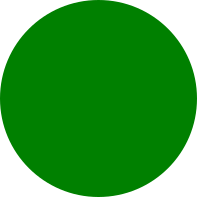
\includegraphics[width=1.5cm]{213.png}};
		\node[](o3) at (2,0){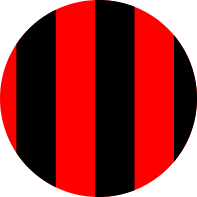
\includegraphics[width=1.5cm]{222.png}};
		
		\draw[dashed, color=orange,line width=1mm] (o3.south west) rectangle ++(1.75cm,1.75cm);
		
		\node[] at ([yshift=10pt]o2.north){Utterance: \textbf{``red"}};
		\end{tikzpicture}
		\subcaption{Another combination, here two red objects differ in texture but share shape.}
	\end{subfigure}
	\hspace*{0.5cm}
	\begin{subfigure}[b]{0.45\linewidth}
		\begin{tikzpicture}
		\node[](o1) at (-2,0){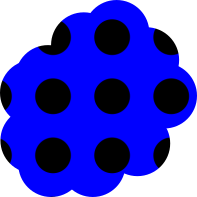
\includegraphics[width=1.5cm]{131.png}};
		\node[](o2) at (0,0){
\includegraphics[width=1.5cm]{112.png}};
		\node[](o3) at (2,0){
\includegraphics[width=1.5cm]{111.png}};
		
		\draw[dashed, color=orange,line width=1mm] (o2.south west) rectangle ++(1.75cm,1.75cm);
		
		\node[] at ([yshift=10pt]o2.north){Utterance: \textbf{``solid"}};
		\end{tikzpicture}
		\subcaption{Two solid objects differ in color but share shape.}
	\end{subfigure}
\caption{In all these examples, the utterance picks out two objects. The picked object has one feature for itself. The other two objects share that feature between them. The last feature is shared by all objects.}
	%21 32 12
\end{figure*}

%class 21 22 12
\begin{figure*}[!ht]
	\centering
	\begin{subfigure}[b]{\linewidth}
		\centering
		\begin{tikzpicture}
		\node[](o1) at (-2,0){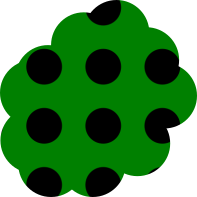
\includegraphics[width=1.5cm]{133.png}};
		\node[](o2) at (0,0){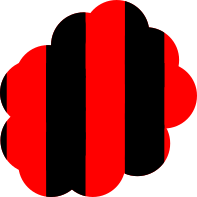
\includegraphics[width=1.5cm]{122.png}};
		\node[](o3) at (2,0){
\includegraphics[width=1.5cm]{232.png}};
		
		\draw[dashed, color=orange,line width=1mm] (o2.south west) rectangle ++(1.75cm,1.75cm);
		
		\node[] at ([yshift=10pt]o2.north){Utterance: \textbf{``red"}};
		\end{tikzpicture}
		\subcaption{The objects can differ in shape, texture, and color. The utterance applies to 2 objects which differ in shape and texture: a striped cloud and a polka-dotted circle. Solid objects or squares are absent in the scene, so we cannot learn whether the listener likes squares or solid objects.}
	\end{subfigure}
	
	\vspace{0.2cm}
	
	\begin{subfigure}[b]{0.45\linewidth}
		\begin{tikzpicture}
		\node[](o1) at (-2,0){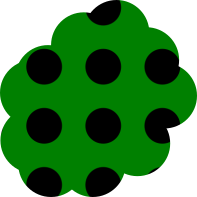
\includegraphics[width=1.5cm]{133.png}};
		\node[](o2) at (0,0){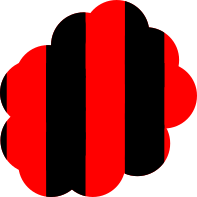
\includegraphics[width=1.5cm]{122.png}};
		\node[](o3) at (2,0){
\includegraphics[width=1.5cm]{232.png}};
		
		\draw[dashed, color=orange,line width=1mm] (o1.south west) rectangle ++(1.75cm,1.75cm);
		
		\node[] at ([yshift=10pt]o2.north){Utterance: \textbf{``polka-dotted"}};
		\end{tikzpicture}
		\subcaption{Another combination, here the polka-dotted objects differ in shape and color.}
	\end{subfigure}
	\hspace*{0.5cm}
	\begin{subfigure}[b]{0.45\linewidth}
		\begin{tikzpicture}
		\node[](o1) at (-2,0){
\includegraphics[width=1.5cm]{212.png}};
		\node[](o2) at (0,0){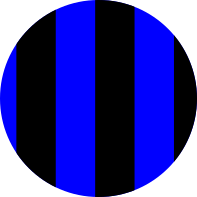
\includegraphics[width=1.5cm]{221.png}};
		\node[](o3) at (2,0){
\includegraphics[width=1.5cm]{311.png}};
		
		\draw[dashed, color=orange,line width=1mm] (o2.south west) rectangle ++(1.75cm,1.75cm);
		
		\node[] at ([yshift=10pt]o2.north){Utterance: \textbf{``circle"}};
		\end{tikzpicture}
		\subcaption{Two circles differ in texture and color.}
	\end{subfigure}
	%21 22 12
	\caption{The utterance always picks out two objects and both objects only share that uttered feature. The third object shares one feature with each of those objects.}
\end{figure*}


%class 32 21 12
\begin{figure*}[!ht]
	\centering
	\begin{subfigure}[b]{\linewidth}
		\centering
		\begin{tikzpicture}
		\node[](o1) at (-2,0){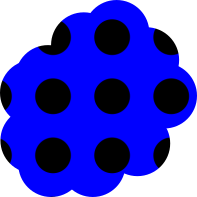
\includegraphics[width=1.5cm]{131.png}};
		\node[](o2) at (0,0){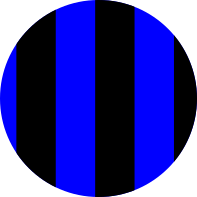
\includegraphics[width=1.5cm]{221.png}};
		\node[](o3) at (2,0){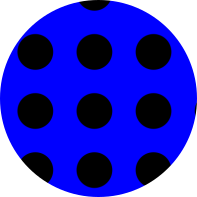
\includegraphics[width=1.5cm]{231.png}};
		
		\draw[dashed, color=orange,line width=1mm] (o1.south west) rectangle ++(1.75cm,1.75cm);
		
		\node[] at ([yshift=10pt]o2.north){Utterance: \textbf{``blue"}};
		\end{tikzpicture}
		\subcaption{The objects can differ in shape, texture, and color. The utterance applies to all 3 objects but they differ in shape and texture. Solid objects or squares are absent here, so we cannot learn whether the listener likes squares or solid objects.}
	\end{subfigure}
	\vspace{0.2cm}
	
	\begin{subfigure}[b]{0.45\linewidth}
		\begin{tikzpicture}
		\node[](o1) at (-2,0){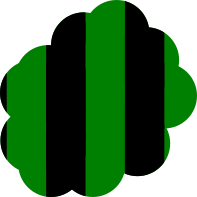
\includegraphics[width=1.5cm]{123.png}};
		\node[](o2) at (0,0){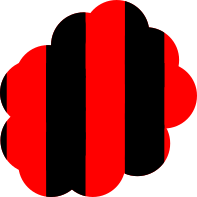
\includegraphics[width=1.5cm]{122.png}};
		\node[](o3) at (2,0){
\includegraphics[width=1.5cm]{112.png}};
		
		\draw[dashed, color=orange,line width=1mm] (o3.south west) rectangle ++(1.75cm,1.75cm);
		
		\node[] at ([yshift=10pt]o2.north){Utterance: \textbf{``cloud"}};
		\end{tikzpicture}
		\subcaption{Another combination, here all objects are clouds but the picked object shares being red with another object.}
	\end{subfigure}
	\hspace*{0.5cm}
	\begin{subfigure}[b]{0.45\linewidth}
		\begin{tikzpicture}
		\node[](o1) at (-2,0){
\includegraphics[width=1.5cm]{311.png}};
		\node[](o2) at (0,0){
\includegraphics[width=1.5cm]{211.png}};
		\node[](o3) at (2,0){
\includegraphics[width=1.5cm]{313.png}};
		
		\draw[dashed, color=orange,line width=1mm] (o2.south west) rectangle ++(1.75cm,1.75cm);
		
		\node[] at ([yshift=10pt]o2.north){Utterance: \textbf{"solid"}};
		\end{tikzpicture}
		\subcaption{All objects are solid, the picked object shares being blue with one object.}
	\end{subfigure}
	%32 21 12
	\caption{Here the utterance picks out all objects. The picked object shares one feature with one other object and has one feature just for itself while the other two objects share it.}
\end{figure*}
	
\end{document}